\section{The chosen approach}

In order to make things easier and to be able to set tangible milestones, the
challenge is split in two logical problems to be solved, one after the
other. The problem is not solved as a whole race, but rather as a trajectory
between a starting point and a gate. This choice of approach is motivated by
the fact that admitedly, if the nearest gate detection is quick and precise,
considering a race as a succession of independent targets to be reached is
theoreticaly a robust solution that can be applied to any environment, with any
obstacles, and of any length.\\

\begin{figure}[h]
	\centering
	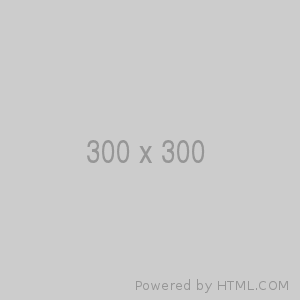
\includegraphics[width=0.5\textwidth]{figure/300x300.png}
	\caption{System diagram.}
	\label{fig:iros}
\end{figure}

Firstly, the perception logic is solved with a deep learning algorithm, most
precisely with a convolutional neural network. However, it has been seen from
the literature review that collecting a dataset for drone racing can be
tedious, and is rarely variate enough to allow for good generalization of the
learning and application in any given environment. In this work, a
semi-synthetic dataset is generated from background images, to provide an
infinite amount of circuit combinations to train the gate recognition network
(more on that in the following chapter).

Being the main research topic of this thesis, this part is given more time and
focus to deliver a more rigourous and in-depth work.\\

\begin{figure}[h]
	\centering
	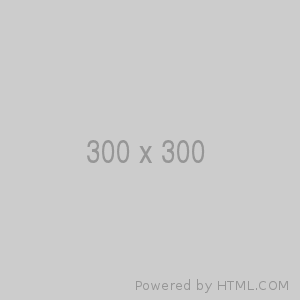
\includegraphics[width=0.5\textwidth]{figure/300x300.png}
	\caption{Block diagram of the perception logic.}
	\label{fig:iros}
\end{figure}

Secondly, the control logic is made as simple as can be, since its purpose is
only to verify the hypothesis proposed for the perception. A state machine is
supervising the flight between the two gates, and utilizes a
Proportional-Integral-Derivative controller to output velocity commands to the
lower-level controller implemented by the manufacturer on the UAV.\\

\begin{figure}[h]
	\centering
	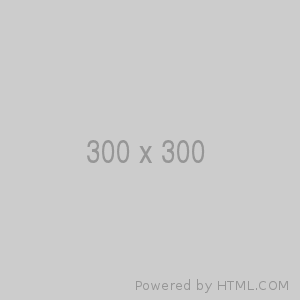
\includegraphics[width=0.5\textwidth]{figure/300x300.png}
	\caption{Block diagram of the control logic.}
	\label{fig:iros}
\end{figure}


As for the drone itself, 

The solution will be implemented iteratively, by gradually increasing the
complexity of the vision algorithms, such that progress can be made even if the
end goal is too difficult to achieve.\\

The project should attempt to fulfill the following goals:

\begin{itemize}
	\item{Recognize gates in the input image}
	\item{Detect and localize the closest gate's center}
	\item{Evaluate the closest gate's orientation and distance}
	\item{Plan a trajectory for the drone to fly across the gate center}
	\item{Refine the trajectory in real time, for an optimal flight time}
	\item{Make the drone follow that trajectory while adjusting in real time}
\end{itemize}
~\\
However, the following functionalities are out of the scope and will be
discarded:

\begin{itemize}
	\item{Detect any other obstacles in the input image}
	\item{Avoid obstacles that are on the drone's trajectory}
	\item{Map and localize the detected gates in world frame}
	\item{Plan a trajectory of a sequence of gates}
	\item{Apply online learning for adaptive racing}
\end{itemize}


\todo{System diagram, framework, ROS and all the shit}
